\documentclass[
a4paper,
10pt,
twoside,
prd,
aps,
nofootinbib,
superscriptaddress,
floatfix,
preprintnumbers,
]{article}


\usepackage{preamble}
\usepackage{titleinfo}

\geometry{ % Set document margins
	top     = 2cm,
	bottom  = 2cm,
	left    = 1cm,
	right   = 1cm
}

\newcommand{\mcols}{2} % Choose number of columns (>= 1)


\bibSetup{refs.bib} % Give references file 
% ===== Format headers & footers =====

\pagestyle{fancy}
\fancyhf{}
\fancyhead[LE,RO]{B. Henke}
\fancyhead[LO]{\headertitle\hspace{0.5cm}\textit{PHY803}}
\fancyhead[RE]{\textit{PHY803}\hspace{0.5cm}\headertitle}
\fancyfoot[RE,LO]{\thepage}

\begin{document}
% \tableofcontents
\titleinf
\maketitle

\begin{abstract}
	
	\noindent
	The purpose of the paper to be summarized here is to calculate the contribution to the muon's anomalous magnetic moment due to hadronic vacuum polatization.
	This is done by analyzing the connected diagrams of up and down quarks.
	Five ensembles are analized with lattice spacings ranging from $a \approx 0.06$ to $0.15$fm.
	In the paper, the up and down quarks are given the same mass ($m_l$), which implies that all pions have the same mass (that of the $\pi^0$).
	From this set up, a light-light connected anomalous magnetic moment of the muon is calculated to be $a_\mu^{ll}(\text{conn.}) = 637.8(8.8) \times 10^{-10}$, which agrees with independent lattice-QCD calculations.
	This value excludes strong-isospin breaking (SIB), electromagnetism, and contributions from quark-disconnected diagrams, so the value is corrected using published lattice-QCD results.
	After the corrections are made, a final value of $a_\mu^{\text{HVP,LO}} = 699(15)_{u,d}(1)_{s,c,b} \times 10^{-10}$ is found.
	This value agrees with experimental data and with \textit{ab-initio} lattice-QCD calculations, and is $1.3\sigma$ below the "no new physics" value of the hadronic-vacuum-polarization contribution inferred from combining theoretical calculations of the other contributions with the Brookhaven National Laboratory (BNL) E821 measurement.
	
\end{abstract}

\startmcols


\section{Introduction}

\begin{figure}[H]
	\centering
	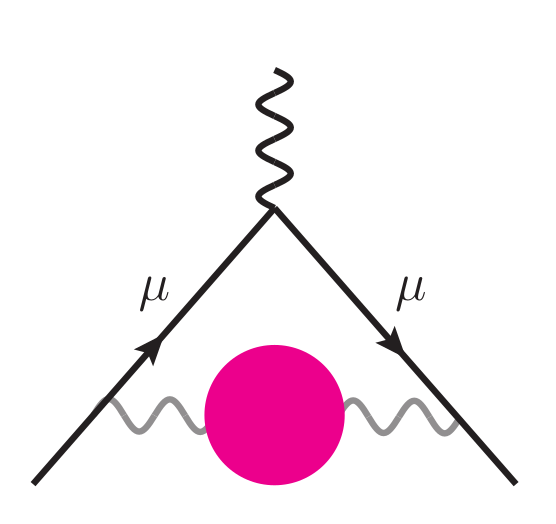
\includegraphics[width=0.75\linewidth]{figures/paperFig1.png}
	\captionsetup{width=0.8\linewidth}
	\caption{%
		Figure 1 from \cite{Davies_2020}.
		It is a Feynmann diagram showing the leading hadronic contribution to the muon $g_\mu-2$.
		The shaded circle signifies a host of different interactions that contribute to the muon's anomalous magnetic moment.
		These fall into two categories: quark-connected and quark-disconnected.
		Quark-connected interactions are where the photon creates a quark-antiquark pair, which iteract and annihilate back into a photon.
		However, if the quark-antiquark pair annihilate into glouns, this is called "quark-disconnected".\cite{Davies_2020}
	}
	\label{fig: paperFig1}
\end{figure}

The anomalous magnetic moment of the muon, $a_\mu$, is an observable in the Standard-Model framework.
It is defined as $(g_\mu − 2)/2$ where the gyromagnetic ratio, $g_\mu$, would have a value of two in a world with no quantum corrections\cite{Davies_2020}.
There are experiments that can measure it very precisely, and there is very good control of the theoretical calculations of this observable\cite{Davies_2020}.
Hence, it can be used to pin down tiny effects of heavy particles on this low-energy observable, and the effects of lighter particles that are similar to that of the heavy particles, but have evaded detection.\cite{Davies_2020}

The objective of this paper is to calculate the contribution of the muon anomalous magnetic moment hadronic vacuum polarization from the connected diagrams of up and down quarks, omitting electromagnetism.
In order to do this, it employs QCD guage-field configurations with dynamical $u,d,s,$ and $c$ quarks and the physical pion mass, and analyze five ensembles with different lattice spacings ($a \approx 0.06$fm to $a \approx 0.15$fm).
The specifications of all five of these ensembles are shown in table \ref{tab: ensemble_specs}
The diagram in figure \ref{fig: paperFig1} shows the general leading hadronic contribution to the muon $g_\mu-2$ that is analyzed in this paper.

\section{Background and Methodology}
The relation between the leading-order hadronic-vacuum-polarization contribution to the muon’s anomalous magnetic moment and the renormalized quark vacuum polarization function $\hat{\Pi}(Q^2) \equiv \Pi(Q^2) - \Pi(0)$, is given by\cite{Davies_2020}
\begin{equation}
	a_\mu^{HVP,LO} = \left(\frac{\alpha}{2}\right)^2 \int_0^\infty \dd{Q^2} K_E (Q^2) \hat{\Pi}(Q^2).
	\label{eq: magmoment}
\end{equation}
The current-current correlation function, which is used throughout the paper to calculate the muon's anomalous magnetic moment is given by\cite{Davies_2020}
\begin{equation}
	G(t) = \frac{1}{27} \int \dd{\vb{x}} \left[4\ev{j_i^u(\vb{x},t)j_i^u(0,0)} + \ev{j_i^d(\vb{x},t),j_i^d(0,0)}\right].
\end{equation}
Using the current-current correlation function, one calculates the quark vacuum polarization function to be\cite{Davies_2020}
\begin{equation}
	\hat{\Pi}(\omega^2) = \frac{4\pi^2}{\omega^2} \int_0^\infty \dd{t} G(t) \left[\omega^2t^2-4\sin[2](\frac{\omega t}{2})\right].
\end{equation}
This can then be used to achieve the goal of the paper, which is to calculate equation \ref{eq: magmoment}.

The traditional and currently still most precise determinations of $a_\mu^{\text{HVP,LO}}$ use dispersive methods to obtain the vacuum-polarization function from experimental “R-ratio” data\cite{Davies_2020}:
\begin{equation}
	\hat{\Pi}(Q^2) = \frac{Q^2}{3} \int_0^\infty \dd{s}\frac{R_\gamma(s)}{s(s+Q^2)},
\end{equation}
where
\begin{equation}
	R_\gamma (s) \equiv \frac{\sigma(e^+e^- \rightarrow \gamma^* \rightarrow \text{hadrons})}{4\pi\alpha(s)^2/(3s)}.
\end{equation}

\section{Lattice-QCD Calculation}
\label{sec: LatCalc}

\begin{table*}[t]
	\centering
	% \makebox[0.9\linewidth]{%
	\resizebox{\textwidth}{!}{%
	% \setlength{\tabcolsep}{1pt}
	\begin{tabular}{ccccccccc}
		\hline\hline
		$\approx a \text{(fm)}$
		& $am_l^{\text{sea}}/am_s^{\text{sea}}/am_c^{\text{sea}}$
		& $w_0/a$
		& $Z_{V,\bar{s}s}$
		& $M_{\pi_5} \text{(MeV)}$
		& $E_{2\pi,\text{min}}\text{(MeV)}$
		& $(L/a)^3\times(T/a)$
		& $N_{\text{conf.}}$
		& $N_{\text{wall}}$
		\\\hline
		0.15 & 0.00235/0.0647/0.831 & 1.13670(50) & 0.9881(10) & 133.04(70) & 640.4(3.4) & $32^3\times 48$ & 997
		& 16\\
		0.15 & 0.002426/0.0673/0.8447 & 1.13215(35) & 0.9881(10) & 134.73(71) & 639.7(3.4) & $32^3 \times 48$ & 9362 & 48 \text{(TSM)}\\
		0.12 & 0.00184/0.0507/0.628 & 1.41490(60) & 0.99220(40) & 132.73(70) & 540.8(3.3) & $48^3 \times 64$ & 998 & 16\\
		0.09 & 0.00120/0.0363/0.432 & 1.95180(70) & 0.99400(50) & 128.34(68) & 524.3(2.8) & $64^3 \times 96$ & 1557 & 16 \text{(TSM)}\\
		0.06 & 0.0008/0.022/0.260 & 3.0170(23) & 0.9941(11) & 134.95(72) & 530.8(2.8) & $96^3 \times 192$ & 1230 & 16 \text{(TSM)}
		\\\hline\hline
	\end{tabular}
	}
	% $
	% \begin{array}{ccccccccc}
		
	% \end{array}
	% $
	% }
	\captionsetup{width=0.8\linewidth}
	\caption{%
		"Table I" from \cite{Davies_2020}.
		These are the parameters of the QCD guage-field ensembles.
		The first column shows the approximate lattice spacing.
		The second lists the bare lattice up, down, strange, and charm sea-quark masses.
		The third, fourth, and fifth columns are values used to compare to other resources\cite{Bazavov_2013,2012,Dowdall_2013,PhysRevD.96.034516}.
		The sixth column shows the lowest-lying noninteracting two-pion energy level that couples to the vector current for each ensemble.
		The seventh column gives the latice volumes.
		Lastly, the two remaining columns give the number of configurations analyzed and the number of random-wall time sources used per configuration.
	}
	\label{tab: ensemble_specs}
\end{table*}

\subsection{Numerical Simulation}
\label{sec: LatCalcA}
A calculation on QCD gauge-field configurations generated by the MILC Collaboration with four flavors of HISQ quarks was performed.
These configurations are isospin-symmetric, i.e., the up and down sea-quark (the virtual quark-antiquark pairs in hadrons) masses are equal with a mass $ m_l = (m_u + m_d)/2 $.

Two of the ensembles listed in table \ref{tab: ensemble_specs} were also used in \cite{PhysRevD.96.034516}:
the $a \approx 0.15$fm ensemble with approximately 1000 configurations and the $a \approx 0.12$fm ensemble.
In addition, a new ensemble is included with $a \approx 0.15$fm and parameters identical to the older $a \approx 0.15$fm physical-mass ensemble, except for having better tuned quark masses.
Thus, comparing this high-statistics ensemble and the older low-statistics one enables us to test our methods for extracting all $ a_\mu^{ll}$(conn.) from noisy data.

On the three newer ensembles analyzed in this work, in addition, a cost-effective variance-reduction technique called the truncated solver method (TSM) was employed, which reduces computational costs by a factor of $>2$.


\subsection{Extraction of Muon Anomaly}
\label{sec: LatCalcB}
\begin{figure}[H]
	\centering
	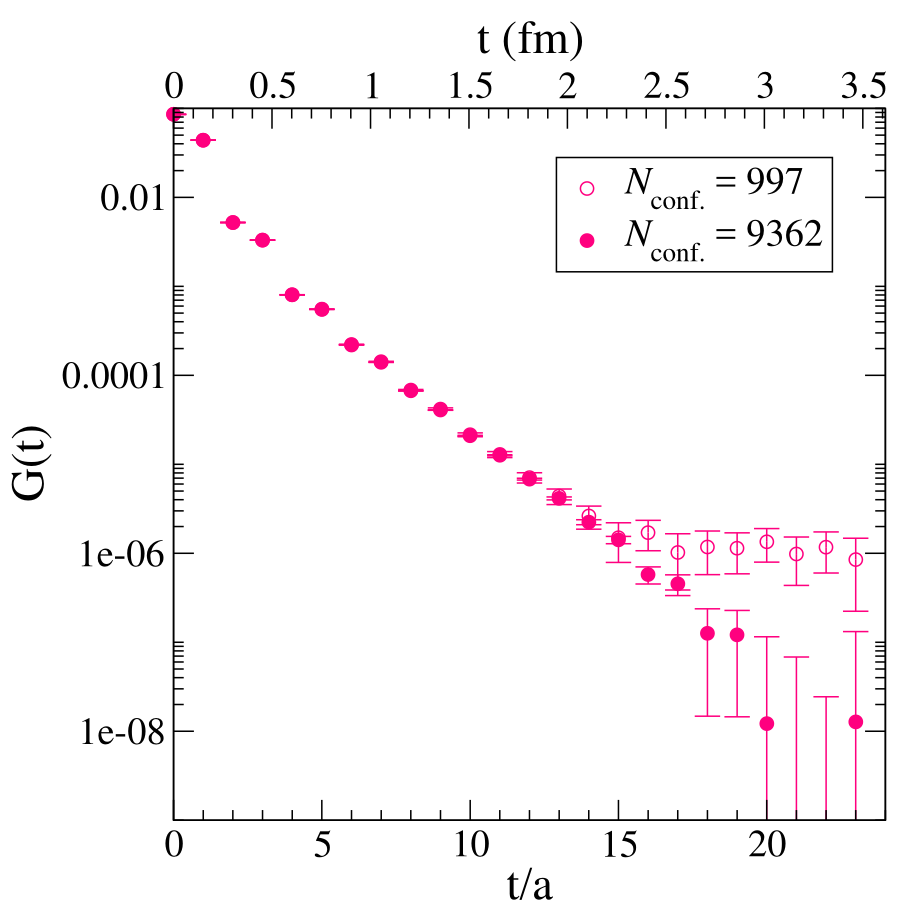
\includegraphics[width=0.75\linewidth]{figures/paperFig2.png}
	\captionsetup{width=0.8\linewidth}
	\caption{%
	Figure 2 from \cite{Davies_2020}.
	This figure shows the local-local vector-current correlator on the two $a \approx 0.15$fm ensembles with similar parameters but differing statistics.
	}
	\label{fig: paperFig2}
\end{figure}

A challenge common to all lattice-QCD calculations
of $a_\mu^{ll}$ (conn.) is the large statistical noise in the vector-current correlator at the physical light-quark mass.
Figure \ref{fig: paperFig2} shows the local-local vector-current correlator $G(t)$ on the two $a \approx 0.15$fm ensembles.
The correlator values at times $t$ and $T-t$ are averaged to increase statistics.
Beyond this range, the data with low statistics become too noisy to yield a reliable estimate of the correlation function.
Several strategies to address the noise problem can used.
In this paper, the same strategy is used as in \cite{PhysRevD.96.034516}.

\subsection{Lattice Corrections and Continuum Extrapolation}
\label{sec: LatCalcC}

Before extrapolating the values obtained for $a_\mu^{ll}$(conn.) in the previous section to zero lattice spacing, the data are corrected for the finite lattice spatial volume and for dis cretization effects from the mass splittings between staggered pions of different tastes.
Both effects arise from one-loop diagrams with $\pi\pi$ intermediate states.

One can test the estimates of the lattice corrections by comparing the results for the Taylor coefficients of the vacuum-polarization function with phenomenological determinations from R-ratio data.
Because the experimental data include all possible diagrammatic contributions, for this test, the full one-loop correction is used, which includes both the connected and disconnected pieces.

\section{Results}
\label{sec: Results}
In this section, the results for $a_\mu^{ll}\text{(conn.)}, \Pi_1^{ll} , \Pi_2^{ll} ,$ and $a_\mu^{\text{HVP,LO}}$ and the slope and curvature of $\hat{\Pi}(Q^2)$ comprehensive error budgets are presented.
There are several types of corrections to the values calculated.
These, along with the found values are shown in table \ref{tab: corrections}.


\subsection{Light-Quark Connected Contribution}

Their numerical calculation of $a_\mu^{ll}$(conn.) and the slope and curvature of the renormalized vacuum-polarization function is with equal up- and down-quark masses, and without electromagnetism.
The results in the isospin-symmetric limit are
\begin{align}
	a_\mu^{ll} \text{(conn.)} &= 637.8(8.8) \times 10^{-10},\label{eq: a rez}\\
	\Pi_1^{ll} \text{(conn.)} &= 0.0932(14) \text{GeV}^2,\\
	\Pi_2^{ll} \text{(conn.)} &= -0.2089(64) \text{GeV}^4.
\end{align}

A total uncertainty of $1.4\%$ on the light-quark connected contribution to $a_\mu^{\text{HVP,LO}}$ in the isospin-symmetric limit without electromagnetism is obtained.

\subsection{Isospin-Breaking, Electromagnetic, and Quark-Disconnected Contributions}
To be able to compare the total summed over all quark flavors with experiment, one needs to correct the result for $a_\mu^{ll}$(conn.) (equation \ref{eq: a rez})

\begin{table*}[b]
	\centering
	\begin{tabular}{cc}
		\hline\hline
		Correction for & Correction value \\\hline
		$\pi\pi$ corrections & $\Delta a_\mu^{\pi\pi}\text{(disc.)} = -12(3) \times 10^{-10}$ \\
		non-$\pi\pi$ corrections & $\Delta a_\mu^{\rho\omega} \text{(disc.)} = -5(5)\times 10^{-10}$ \\
		Strong-Isospin Breaking (SIB) corrections & $\Delta a_\mu^{ud} \text{(SIB)} = 10(10) \times 10^{-10}$ \\
		QED corrections & $\Delta a_\mu^{ud}\text{(QED)} = 0(5) \times 10^{-10}$\\\hline\hline
	\end{tabular}
	\captionsetup{width=0.8\linewidth}
	\caption{%
		This table shows each of the light-quark corrections to equation \ref{eq: a rez}.
		Summing these with equation \ref{eq: a rez}, and corrections for heavy-quarks (see section \ref{sec: Results}\ref{sec: total LO contribution}), gives the hadron-vacuum-polarization contribution to the muon's anomalous magnetic moment, $a_\mu^{\text{HVP,LO}}$.
	}
	\label{tab: corrections}
\end{table*}

\subsubsection{$\pi\pi$ Corrections}
A large part of the isospin, electromagnetic, and quark-disconnected corrections comes from diagrams in figure \ref{fig: paperFig1} with $\pi\pi$ intermediate states.
These corrections can be estimated using the leading term in the chiral model.

Achieved was a total $\pi\pi$ correction to $a_\mu^{\text{HVP,LO}}$ from strong-isospin breaking, electromagnetism, and quark-disconnected diagrams
\begin{equation}
	\Delta a_\mu^{\pi\pi}\text{(disc.)} = -12(3) \times 10^{-10}.
	\label{eq: pipi}
\end{equation}

\subsubsection{Residual Light-Quark Disconnect Corrections}

There are also quark-line disconnected corrections to $a_\mu^{\text{HVP,LO}}$ that have nothing to do with the $\pi\pi$ contribution.
One can estimate these by examining the contributions to the anomaly from the $\rho$ and $\omega$ mesons.
These resonances, together, account for almost $80\%$ of the total $a_\mu^{\text{HVP,LO}}$.
A disconnected contribution from non-$\pi\pi$ states is achieved:
\begin{equation}
	\Delta a_\mu^{\rho\omega} \text{(disc.)} = -5(5)\times 10^{-10}.
	\label{eq: rhoomega}
\end{equation}

\subsubsection{Residual Strong-Isospin Breaking Corrections}

The effects from QCD-isospin breaking (i.e., quark-mass differences) and QED are intertwined both in nature and in lattice-QCD simulations.
In the paper, the residual strong-isospin correctioon to $a_\mu^{\text{HVP,LO}}$ is defined as the shift relative to the isospin-symmetric value $a_\mu^{ll}$(conn.) that results when the bare $u$ and $d$ quark masses are retuned separately.
A relative correction of $\delta a_\mu^{\text{HVP,LO}}\text{(SIB)} = 1.5(7)\%$ was found, which translates to an absolute correction of $\Delta a_\mu^{\text{HVP,LO}}\text{(SIB)}=9.5(4.5) \times 10^{-10}$, when commined with $a_\mu^{ll}$(conn.) from \ref{eq: a rez}.
It is concluded by increasing the errors on their initial estimate of the total residual correction from strong-isospin breaking to allow for disconnected contributions of a commensurate size, giving
\begin{equation}
	\Delta a_\mu^{ud} \text{(SIB)} = 10(10) \times 10^{-10}.
	\label{eq: ud SIB}
\end{equation}


\subsubsection{Residual QED Corrections}
The residual corrections from QED is estimated, beyond those accounted for above, via power-counting to be of order $α \sim 1\%$.
This yields an estimate for the absolute correction to $a_\mu^{\text{HVP,LO}}$ of
\begin{equation}
	\Delta a_\mu^{ud}\text{(QED)} = 0(5) \times 10^{-10}.
	\label{eq: ud QED}
\end{equation}

\subsubsection{Total Contribution from $u/d$ Quarks}

Summing the corrections from equations \ref{eq: pipi} and equations \ref{eq: rhoomega}-\ref{eq: ud QED} gives the total correction from strong-isospin breaking, QED, and quark-disconnectedcontributions:
\begin{equation}
	\Delta a_\mu^{ud} \text{(SIB,QED,disc.)} = -7(13)\times 10^{-10}.
\end{equation}
Adding this to $a_\mu^{ll}$(conn.) (equation \ref{eq: a rez}) gives the total contribution to $a_\mu^{HVP,LO}$ from light quarks:
\begin{equation}
	a_\mu^{ud} = 630.8(8.8)(13) \times 10^{-10},
	\label{eq: a ud TOT}
\end{equation}
where the first error is from $a_\mu^{ll}$(conn.) and the second error is from $\Delta a_\mu^{ud}$.

\subsection{Total Leading-Order Contribution}
\label{sec: total LO contribution}

Finally, to obtain the total leading-order hadronic vacuum polarization contribution to $a_\mu$, the contributions from heavy flavors are added to $a_\mu^{ud}$ (equation \ref{eq: a ud TOT}):
\begin{equation}
	a_\mu^{\text{HVP,LO}} = 699(15)_{u,d} (1)_{s,c,b} \times 10^{-10}.
	\label{eq: a_mu tot}
\end{equation}
Disconnected contributions from these quarks are expected to be negligible compared with our other uncertainties.


\section{Conclusion}

The final value found for the leading-order hadronic-vacuum-polarization contribution to $a_\mu$ (equation \ref{eq: a_mu tot}) agrees with other lattice-QCD calculations and phenomenological analyses of experimental $R$-ratio data, and has comparible error\cite{Davies_2020}.
This result is $1.3\sigma$ below the "no new physics" value, with about twice the uncertainty.
Due to this high uncertainty, one cannot draw any conclusions on the presence of new physics\cite{Davies_2020}.

\nocite{*}
\printbib


\stopmcols


\end{document}

